%Still, even given MiniHack's increased complexity and task difficulty compared to baba-is-ai (baseline performance of 10\% on MiniHack vs 33\% on baba-is-ai), 

\centering
\begin{tabular}{cc>{\raggedright\arraybackslash}p{6cm}}
\toprule
\multicolumn{1}{c}{\textbf{}} & 
\multicolumn{1}{c}{\textbf{Turn}} & 
\multicolumn{1}{c}{\textbf{Description}} \\
\midrule
\rowcolor{gray!10} 
\includegraphics[scale=0.07]{figs/emojis/mini_1.png} & 0 & Target Navigation Effectiveness \\
\midrule
\rowcolor{gray!10} 
\includegraphics[scale=0.07]{figs/emojis/mini_2.png} & 0 & Efficient Exploration and Map Memory Utilization \\
\midrule
\rowcolor{gray!10} 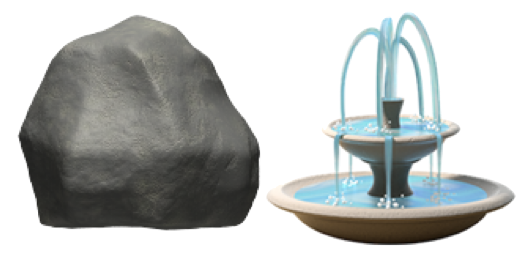
\includegraphics[scale=0.07]{figs/emojis/mini_3.png} & 0 & Hazard Awareness and Equipment Utilization \\
\midrule
\rowcolor{gray!10} 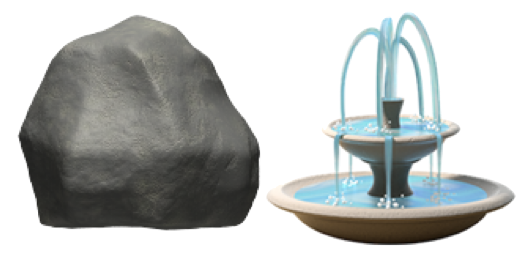
\includegraphics[scale=0.07]{figs/emojis/mini_4.png} & 0 & Boulder Manipulation Strategy \\
\midrule
\rowcolor{gray!10} 
\includegraphics[scale=0.07]{figs/emojis/mini_5.png} & 0 & Combat Engagement and Survival \\
\midrule
\rowcolor{gray!10} 
\includegraphics[scale=0.07]{figs/emojis/mini_6.png} & 0 & Role-Specific Ability Utilization  \\
\midrule
\rowcolor{gray!30} 
\includegraphics[scale=0.07]{figs/emojis/mini_7.png} & 1 & Spatial Awareness and Interpretation  \\
\midrule
\rowcolor{gray!30} 
\includegraphics[scale=0.07]{figs/emojis/mini_8.png} & 1 & Object Pickup Efficiency \\
\midrule
\rowcolor{gray!60} 
\includegraphics[scale=0.07]{figs/emojis/mini_9.png} & 2 & Giant Rats Encounter Handling \\
\bottomrule
\end{tabular}

\caption{\raggedright Metrics and Turn of Induction for MiniHack}
\label{tab:metrics_mini}



\begin{flushleft}

The induced metrics and the agent's per-task performance are shown in Table \ref{tab:metrics_mini} and Table \ref{tab:metric_mini_perf}, respectively. A substantial improvement in the agent's task completion performance is observed from \emph{Iteration 1} to \emph{Iteration 2}, with the agent achieving both a higher environment score and trajectory performance on the held-out tasks compared to the baseline agent. Specifically, the agent's performance on metrics increased correspondingly to code changes, like 
\includegraphics[ scale=0.05]{figs/emojis/mini_1.png} improving from $16.67\%$ to $41.67\%$, demonstrating the utility of AutoLibra for fine-grained agent improvement. This is discussed in more detail in the following sections.

\subsection{Extracted Metrics and Improvements}
The metrics induced by AutoLibra (Table \ref{tab:metrics_mini}) capture the behavior of the agent through all iterations, with coverage of 83\% at \emph{Iteration 0} to 88\% at \emph{Iteration 2}. Due to the diversity of tasks, metrics pertain to one or two tasks, matching the expectation that AutoLibra should generate fine-grained metrics. Notably, the metrics generated at \emph{Iteration 0} are nearly comprehensive as they demonstrate good coverage of all four MiniHack tasks, while the later metrics were found to specifically describe detailed behaviors for targeting one task each. Code changes were selected to specifically target improvements in given metrics, and as seen in Table \ref{tab:metric_mini_perf}, the agent's performance on the targeted metric improved significantly in the iteration following the code change. This demonstrates the utility of AutoLibra for fine-grained agent improvement, as well as the human interpretability of the induced metrics. On the other hand, some metrics remain unchanged over iterations. The unchanged metrics are 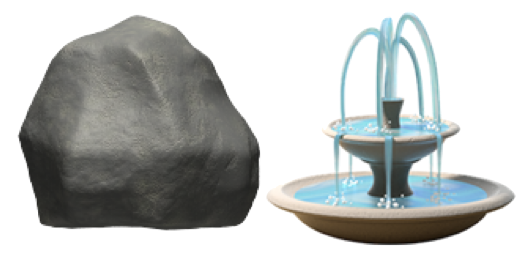
\includegraphics[ scale=0.05]{figs/emojis/mini_3.png}, 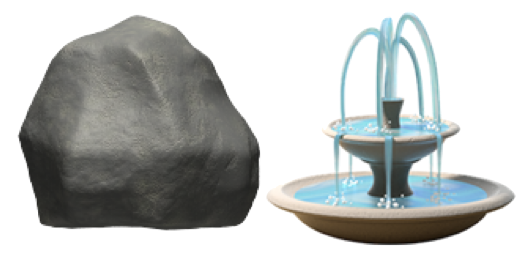
\includegraphics[ scale=0.05]{figs/emojis/mini_4.png}, 
\includegraphics[ scale=0.05]{figs/emojis/mini_6.png}, and 
\includegraphics[ scale=0.05]{figs/emojis/mini_8.png}. This indicates that simply coding might not be sufficient if the gap between the agent's capability and the task's complexity is too significant.

\textbf{Iteration 0}
The agent's behavior is stochastic and repetitive, with no utilization of memory, planning, and goal awareness. Although the agent has reasoning before taking action, the decided action shows no correlation with the goal or the environment. \texttt{Target Navigation Effectiveness} 
\includegraphics[ scale=0.05]{figs/emojis/mini_1.png} was identified as the core metric that evaluates the performance of all tasks except Boxoban. As all three other tasks require the agent to explore the target exit stairs, 
\includegraphics[ scale=0.05]{figs/emojis/mini_1.png} serves as the fundamental test of the agent's goal awareness for these tasks. Since Boxoban has a different winning condition, \texttt{Boulder Manipulation Strategy} 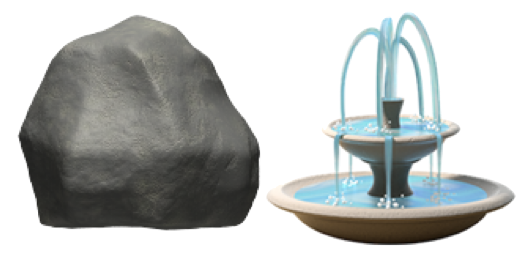
\includegraphics[ scale=0.05]{figs/emojis/mini_4.png} induced in this iteration targets describing the overall goal awareness for the agent in Boxoban environment. The remaining four metrics each cover two to three tasks on a more detailed level.

Based on the metrics induced in \emph{Iteration 0}, several changes to the agent code were implemented:
\begin{itemize}
    \item Augmentation of subtask-level behavioral restriction guidance with the single-shot example, targeting improvement of \texttt{Boulder Manipulation Strategy} 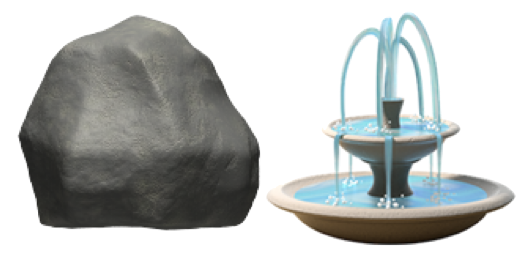
\includegraphics[ scale=0.05]{figs/emojis/mini_4.png}, \texttt{Combat Engagement and Survival} 
\includegraphics[ scale=0.05]{figs/emojis/mini_5.png}, and \texttt{Hazard Awareness and Equipment Utilization} 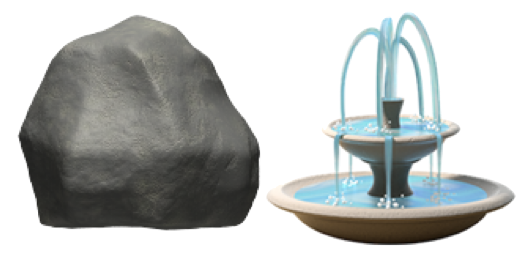
\includegraphics[ scale=0.05]{figs/emojis/mini_3.png}.
    \item Meta-prompting by providing subtask instructions targeting improvement of \texttt{Role-Specific Ability Utilization} 
\includegraphics[ scale=0.05]{figs/emojis/mini_6.png}.
    \item Augmentation of subtask-level winning strategy with few-shot example, targeting improvement of \texttt{Target Navigation Effectiveness} 
\includegraphics[ scale=0.05]{figs/emojis/mini_1.png} and  \texttt{Efficient Exploration and Map Memory Utilization} 
\includegraphics[ scale=0.05]{figs/emojis/mini_2.png}.
\end{itemize}

\textbf{Iteration 1}
The changes made after \emph{Iteration 0} did not yield substantial improvements in agent task completion performance, but behavior changes matching the metrics were observed and insights on prompt improvements were obtained. A decrease in 
\includegraphics[ scale=0.05]{figs/emojis/mini_1.png} performance of 8.3\% was observed between \emph{Iteration 0} and \emph{Iteration 1}, indicating that the code changes confuse the agent which reduces their capability of goal recognition, and the same reduction is also observed for 
\includegraphics[ scale=0.05]{figs/emojis/mini_2.png}. Three causes of these reductions are recognized. Firstly, the overly simplified strategy for MazeWalk provides no positive intuitions for the agent when loops exist in the map. Secondly, the seemingly straightforward behavioral restrictions with examples do not appear sufficient enough for the agent to avoid false action as the agent failed to comprehend the map thorough enough. Thirdly, the randomness of Quest is so high that existing guidance fails to cover new randomly generated situations. Based on \emph{Iteration 1's} result, MazeWalk and Corridor Fight both appear solvable given a more optimal strategy, and Quest and Boxoban, given their high randomness and complexity, do not appear easily solvable, so providing more examples seem to be the only direction of improvement. Moreover, two new metrics are induced, one focusing on Corridor Fight and the other focusing on Quest. 

Based on the metrics induced in \emph{Iteration 1}, new changes are listed below:
\begin{itemize}
    \item Augmentation of existing subtask-level advanced strategy with step-by-step decision-making instructions and few-shot examples, targeting improvement of  \texttt{Target Navigation Effectiveness} 
\includegraphics[ scale=0.05]{figs/emojis/mini_1.png} and  \texttt{Efficient Exploration and Map Memory Utilization} 
\includegraphics[ scale=0.05]{figs/emojis/mini_2.png}.
    \item Augmentation of existing subtask-level strategy with corner cases handling guidance and few-shot examples, targeting improvement of \texttt{Combat Engagement and Survival} 
\includegraphics[ scale=0.05]{figs/emojis/mini_5.png}, \texttt{Hazard Awareness and Equipment Utilization} 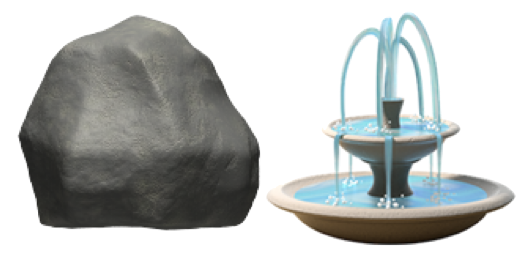
\includegraphics[ scale=0.05]{figs/emojis/mini_3.png}, and \texttt{Spatial Awareness and Interpretation} 
\includegraphics[ scale=0.05]{figs/emojis/mini_7.png}.
    \item Augmentation of existing few-shot examples with a full trajectory of the complete winning task, targeting improvement of \texttt{Boulder Manipulation Strategy} 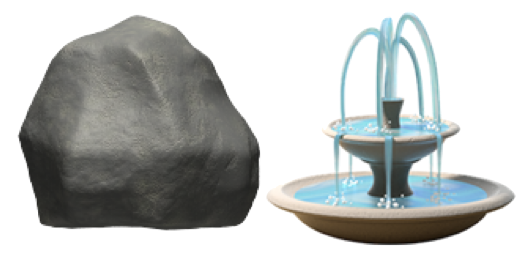
\includegraphics[ scale=0.05]{figs/emojis/mini_4.png}.
    \item Meta-prompting by providing more in-depth subtask instructions, targeting improvement of \texttt{Role-Specific Ability Utilization} 
\includegraphics[ scale=0.05]{figs/emojis/mini_6.png} and \texttt{Object Pickup Efficiency} 
\includegraphics[ scale=0.05]{figs/emojis/mini_8.png}.
\end{itemize}


\textbf{Iteration 2}
We observe a significant increase in 
\includegraphics[ scale=0.05]{figs/emojis/mini_1.png} and 
\includegraphics[ scale=0.05]{figs/emojis/mini_2.png} indicating the code changes successfully improve agent's ability in goal awareness and goal reaching efficiency. Based on task-level observation, the agent succeeded in most MazeWalk and Corridor Fight tasks. The large increase in 
\includegraphics[ scale=0.05]{figs/emojis/mini_5.png} and 
\includegraphics[ scale=0.05]{figs/emojis/mini_7.png} shows the agent's strong performance in the Corridor Fight task. More specifically, the agent now demonstrates both the capability of choosing optimal action based on its current location and the capability of strategically handling dangerous enemies—giant rats—in an emergency. The new induced metric also further proves the agent's rat-handling ability. For instance, when the agent encounters multiple rats at the same time, it will immediately retreat to the middle of the single-way corridor to engage rats in combat individually. By doing so, the agent can easily beat rats one by one and navigate to the goal without danger. However, as all the remaining metrics show no improvements, we also observe the agent's poor performance on Boxoban and Quest. This result shows that our current targeting improvement strategy of adding abundant few-shot examples does not seem effective given the gap between the agent's reasoning ability and the high randomness and complexity of Boxoban and Quest. For example, despite more than ten examples of pushing a boulder to a dead corner, a prohibited behavior has been presented, the agent will still randomly push a boulder to the L-shaped dead corner formed by two walls which causes this boulder to become immovable.


\subsection{Held-Out Task Performance}
For the held-out tasks, the agent task completion rate improved from \emph{Iteration 0} to \emph{Iteration 2}, with scores from 0\% to 25\%. This result further proves that the improvements realized by AutoLibra are generalizable to unseen tasks. However, some failed cases also provide valuable insights into prospective future iterations. For instance, the complete set of Corridor tasks consists of scenarios where the target downstairs may be located west of the agent’s starting point, unlike Corridor Fight, where the target always lies to the east. Consequently, an instruction that rigidly directs the agent to explore only eastward fails to generalize to the broader Corridor tasks. This outcome underscores the importance of crafting instructions that are specific yet flexible: they should provide sufficiently detailed, high-level strategies without relying on overly prescriptive, task-specific steps. By focusing on generalizable principles rather than rigid directions, the agent is better equipped to adapt to a wider range of scenarios while still benefiting from structured guidance. The agent's performance on the held-out tasks is shown in Table \ref{tab:heldout_mini}.

\end{flushleft}


